\begin{table*}[!t]
	\centering
\caption{Declare \textsf{templates} illustrated as exemplifying clauses. $A\wedge p$ ($B\wedge q$) represents the \textit{activation} (\textit{target}) condition, $A$ ($B$) denotes the activity label, and $p$ ($q$) is the data payload condition.}\label{tab:dt}
\resizebox{\textwidth}{!}{\begin{tabular}{c|l|p{9cm}|l}
	\toprule
	Type & Exemplifying clause ($c_l$) & Natural Language Specification for Traces & \LTLf Semantics ($\llbracket c_l \rrbracket$)\\
	\midrule
	 \parbox[t]{2mm}{\multirow{4}{*}{\rotatebox[origin=c]{90}{\textit{Simple}}}} & \textsf{Init($A,p$)} & The trace should start with an activation & $A\wedge p$\\
	 & \textsf{Exists($A,p,n$)} & Activations should occur at least $n$ times & $\Future(A\wedge p \wedge \Next (\llbracket\textsf{Exists} (A,p,n-1)\rrbracket))$\\
	 & \textsf{Absence($A,p,n+1$)}  & Activations should occur at most $n$ times & $\neg \llbracket\textsf{Exists}$($A,p,n+1$)$\rrbracket$\\
	 & \textsf{Precedence($A,p,B,q$)}  & Events preceding the activations should not satisfy the target & $\WeakUntil{\neg(B\wedge p)}{(A\wedge p)}$\\
	 \midrule
	 \parbox[t]{2mm}{\multirow{12}{*}{\rotatebox[origin=c]{90}{\textit{(Mutual) Correlation}}}} 	 & \textsf{ChainPrecedence($A,p,B,q$) }  & The activation is immediately preceded by the target. & $\Globally(\Next(A\wedge p)\Rightarrow (B\wedge q))$\\
	& \textsf{Choice($A,p,B,q$) }  & Either the activation or the target condition must appear. & $\Future(A\wedge p)\vee\Future(B\wedge q)$ \\
	 & \textsf{Response($A,p,B,q$) } & The activation is either followed by or simultaneous to  the target. & $\Globally((A\wedge p)\Rightarrow\Future(B\wedge q))$ \\
	 & \textsf{ChainResponse($A,p,B,q$) }  & The activation is immediately followed by the target. & $\Globally((A\wedge p)\Rightarrow \Next(B\wedge q))$\\
	 & \textsf{RespExistence($A,p,B,q$) }  & The activation requires the existence of the target.& $\Future(A\wedge p)\Rightarrow\Future(B\wedge q)$ \\
	 & \textsf{ExlChoice($A,p,B,q$) } & Either the activation \texttt{xor} the target happen. & $(\Future(A\wedge p)\vee \Future(B\wedge q))\wedge \llbracket\DeclareClause{NotCoExistence}{A}{p}{B}{q}\rrbracket$\\ 
	 & \textsf{CoExistence($A,p,B,q$) }  & \textsf{RespExistence}, and vice versa. & $ \llbracket\DeclareClause{RespExistence}{A}{p}{B}{q}\rrbracket\wedge \llbracket\DeclareClause{RespExistence}{B}{q}{A}{p}\rrbracket$\\
	 & \textsf{Succession($A,p,B,q$) }  & The target should only follow the activation. & $\llbracket\DeclareClause{Precedence}{A}{p}{B}{q}\rrbracket\wedge \llbracket\DeclareClause{Response}{A}{p}{B}{q}\rrbracket$\\

	 & \textsf{ChainSuccession($A,p,B,q$) }  & Activation immediately follows the target, and the target immediately preceeds the activation. & $\Globally((A\wedge p)\Leftrightarrow\Next(B\wedge q))$\\
	 & \textsf{AltResponse($A,p,B,q$) }  & If an activation occurs, no other activations must happen until the target occurs.  & $\Globally((A\wedge p)\Rightarrow(\DUntil{\neg(A\wedge p)}{(B\wedge q)}))$\\
	 & \textsf{AltPrecedence($A,p,B,q$) }  & Every activation must be preceded by an target, without any other
	 activation in between &   $\llbracket\DeclareClause{Precedence}{A}{p}{B}{q}\rrbracket\wedge \Globally((A\wedge p)\Rightarrow \Next(\WeakUntil{\neg(A\wedge p)}{(B\wedge q)})$\\
	 \midrule
	 
	 \parbox[t]{2mm}{\multirow{2}{*}{\rotatebox[origin=c]{90}{\textit{Not.}}}} & \textsf{NotCoExistence($A,p,B,q$) } & The activation \texttt{nand} the target happen.&  $\neg(\Future(A\wedge p)\wedge\Future(B\wedge q))$\\
	 & \textsf{NotSuccession($A,p,B,q$)} & The activation requires that no target condition should follow.& $\Globally((A\wedge p)\Rightarrow \neg\Future(B\wedge q))$ \\
	 \bottomrule
\end{tabular}}
\end{table*} 


\paragraph*{Conformance Checking}\label{sec:DAD} Temporal declarative languages 
pinpoint recurring temporal patterns in highly variable scenarios so as to describe them compactly for both machines and humans \cite{PichlerWZPMR11}.
%model highly variable scenarios, where state machines provide complicated graph models that can be hardly understandable by the common business stake-holder \cite{PichlerWZPMR11}. 
Every single temporal pattern is expressed through \textit{templates} (i.e., an abstract parameterized property: Table \ref{tab:dt} column 2), which are then instantiated on a set of real activation, target, or correlation conditions. We can then categorize each Declare template from \cite{Li2020} by means of these conditions and the ability to express correlations between two temporally distant events happening in one %same timeline (\textit{
trace: %}) 
simple
 templates (Table \ref{tab:dt}, rows 1-3) only involving activation conditions; (mutual)
 correlation templates (rows from 4 to 15), which describe a dependency between two
activation and target conditions, thus including correlations between the two; and negative relation templates (last 2 rows), which describe a negative
dependency between two events in correlation. %Please observe that, 
Despite %some of 
these templates may appear quite similar, but they generate completely different finite state machines, thus suggesting that these conditions are not interchangeable\footnote{\url{http://ltlf2dfa.diag.uniroma1.it/}}. 
\figurename~\ref{fig:comparison} exemplifies the behavioural difference between two clauses differing only on the template of choice.
As a semantics, %formal basis for specifying temporal patterns, 
Declare adopts %the customary choice of of 
Linear Temporal Logic over finite traces (\LTLf), which interprets formulae over an unbounded, yet finite linear sequence of states. %In the context of this paper, consistently with the literature on business
% process execution traces, we make the simplifying assumption that in each point of the sequence, one and only one
%element from $\Sigma$ holds. 
Given a trace $\sigma^i$, the evaluation of a formula $\varphi$ is done in a given state (i.e., event id, or position) of the trace, and we use the notation $\sigma^i_j\vDash\varphi$ to express that $\varphi$ holds starting from the $j$-th event of the $i$-th trace. We also use $\sigma^i\vDash\varphi$ as a shortcut notation for $\sigma^i_0\vDash\varphi$.  %and, consequently, logically captures the
 %notion of conformance of $\sigma$ against $\varphi$. 
 %We say that $\varphi$ is \textit{satisfiable} if it admits at least one conforming trace. 
 This
 denotes that the \underline{entire} trace $\sigma^i$ \textit{satisfies} $\varphi$. Given that a Declare Model  is composed of a set of clauses $\mathcal{M}=\Set{c_l}_{l\leq n,n\in\mathbb{N}}$ which have to be contemporarily satisfied in order to be true, we say that a trace $\sigma^i$ is \textit{conformant} to a model if such a trace satisfies the  \LTLf semantics $\llbracket c_l\rrbracket$ associated to each clause\footnote{More formally, $\sigma^i\vDash\mathcal{M}\Leftrightarrow \forall c_l\in \mathcal{M}. \sigma^i\vDash\llbracket c_l\rrbracket$.} $c_l$. Therefore, the \textsc{Maximum-SATisfiability problem} (Max-SAT) for each trace counts the ratio between the satisfied clauses over the whole model size.
 An \LTLf formula $\varphi$ is built by extending propositional logic with temporal operators in bold: \[\varphi:=\textsf{A}\wedge p\gsep\neg \varphi\gsep\varphi\vee \varphi'\gsep\varphi\wedge\varphi'\gsep\Next{\varphi}\gsep\Globally{\varphi}\gsep\Future{\varphi}\gsep\DUntil{\varphi}{\varphi'}\] where ne\textbf{X}t ($\Next{\varphi}$) denotes that the condition $\varphi$ should occur from the next state, \textbf{G}lobally ($\Globally{\varphi}$) denotes that the condition has to hold on the entire subsequent path, \textbf{F}uture ($\Future{\varphi}$) denotes that the condition should occur somewhere on the subsequent path, and \textbf{U}ntil as $\DUntil{\varphi}{\varphi'}$ denotes that $\varphi$ has to hold at least until $\varphi'$ becomes true, either at the current or a future state. Generally, binary operators bridge activation and target conditions appearing in two distinct sub-formul\ae. Some operators can be seen as syntactic sugar: \textbf{W}eakUntil is denoted as  $\WeakUntil{\varphi}{\varphi'}:=\DUntil{\varphi}{\varphi'}\vee\Globally{\varphi}$, while the implication can be rewritten as $\varphi\Rightarrow\varphi':=(\neg \varphi)\vee (\varphi\wedge \varphi')$. Similarly to relational algebra, these operators also support equivalence rules, thus allowing to rewrite a given \LTLf expression in an equivalent one that might be more efficient to compute.

\begin{figure}[!t]
	\centering

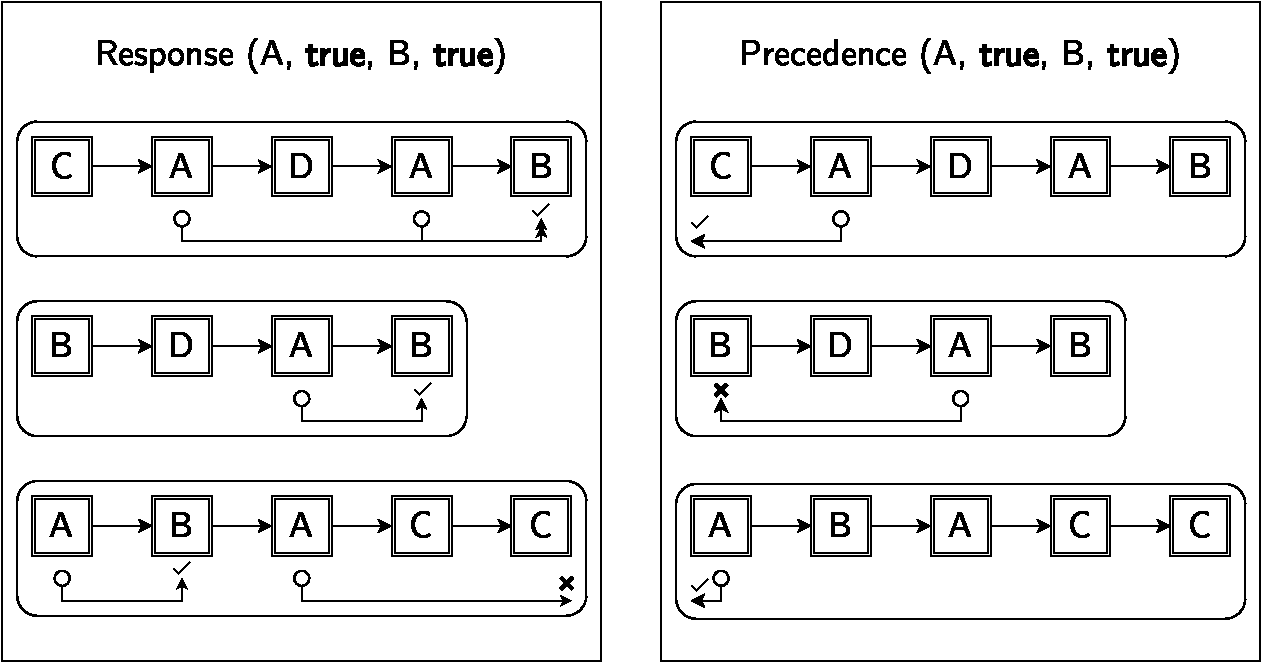
\includegraphics[width=\linewidth]{images/ActivationTargetExample.pdf}
	%	\begin{subfigure}{.27\columnwidth}
		%		\resizebox{\textwidth}{!}{\begin{tabular}{c c} 
				%				\hline
				%				Label & Event \\ 
				%				\hline
				%				\it{a\_a} & audit\_analysis \\
				%				\it{e\_p} & equipment\_purchase \\
				%				\it{p\_r} & patient\_registered \\
				%				\it{p\_d} & patient\_dismissed \\
				%				\hline 
				%		\end{tabular}}
		%	\end{subfigure}
	%\caption{Two exemplifying clauses distinguishing \textsf{Response} and \textsf{Precedence} behaviours. Traces are represented as temporally ordered events associated to activity labels (boxed). Activation  (or target) conditions are here circled (or ticked/crossed). Ticks (or crosses) indicate a (un)successful match of a target condition. For all activations there must be an un-failing target condition; for precedence, we shall consider at most one activation (\S\ref{sec:DAD}). These conditions require the usage of multiple join tests per trace.}
	\caption{Traces describing the events generated by each hospital unit: those are temporally ordered events associated to \textit{activity labels} (boxed). Activated  (or targeted) events here circled (or ticked/crossed). Ticks (or crosses) indicate a (un)successful match of a target condition.}
	\label{fig:comparison}
\end{figure}
Despite this formulation has been already extended so to support correlation constraints \cite{BurattinMS16}, such a solution is affected by the following two deficiencies: first, correlation conditions have to be represented alongside the target condition levels, thus hampering the exploitation of efficient relational database algorithms for correlation conditions via joins. Furthermore, these operators can only assess the validity of one trace at a time while, on the other hand, we might need to assess the satisfiability of multiple traces at the same time by composing partial results returned by every single operator. These operators cannot be directly exploited as query operators, where multiple traces are considered contemporarily. %similarly to the relational algebra operators for relational databases. 
For this reasons, we propose a reformulation of such operators in \S\ref{sec:xltlf} (\xLTLf). 
